% A feasible set of five jobs on two second-stage machines, with the first stage running
% the jobs in earliest-start-time order. Adapted from the slide "Key Observations".
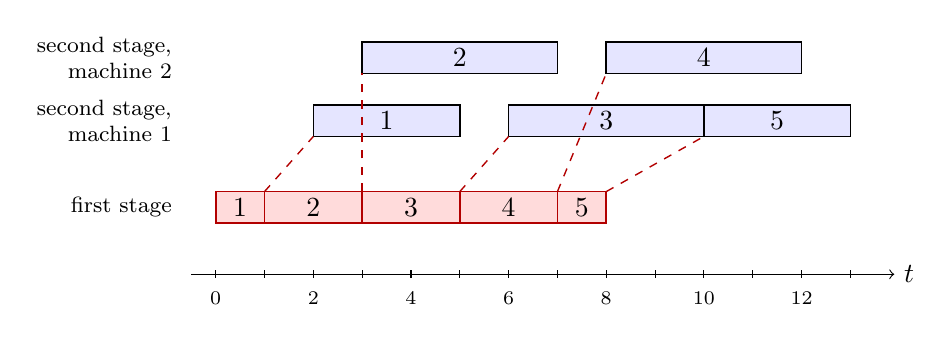
\begin{tikzpicture}[x=0.62cm,y=1cm]
\def\h{0.2}
\colorlet{prep}{red!70!black}
\tikzset{sop/.style={draw,fill=blue!10,line width=0.6pt},
         fop/.style={draw=prep,fill=red!14,line width=0.6pt}}

% the time axis
\draw[->] (-0.5,-0.55) -- (13.9,-0.55) node[right] {$t$};
\foreach \x in {0,1,...,13} \draw (\x,-0.5) -- (\x,-0.6);
\foreach \x in {0,2,4,6,8,10,12} \node[font=\scriptsize] at (\x,-0.85) {\x};

% row labels
\node[anchor=east,font=\footnotesize,align=right] at (-0.7,0.3) {first stage};
\node[anchor=east,font=\footnotesize,align=right] at (-0.7,1.4) {second stage,\\machine 1};
\node[anchor=east,font=\footnotesize,align=right] at (-0.7,2.2) {second stage,\\machine 2};

% second operations: job / start s_j / due date d_j / row
\foreach \j/\s/\d/\y in {1/2/5/1.4, 2/3/7/2.2, 3/6/10/1.4, 4/8/12/2.2, 5/10/13/1.4}
    \draw[sop] (\s,\y-\h) rectangle (\d,\y+\h) node[midway] {$\j$};

% first operations in earliest-start-time order, each ending by the start time s_j
\foreach \j/\a/\b/\s/\y in {1/0/1/2/1.4, 2/1/3/3/2.2, 3/3/5/6/1.4, 4/5/7/8/2.2, 5/7/8/10/1.4}
{
    \draw[fop] (\a,0.3-\h) rectangle (\b,0.3+\h) node[midway] {$\j$};
    \draw[dashed,prep,line width=0.5pt] (\b,0.3+\h) -- (\s,\y-\h);
}
\end{tikzpicture}
